\section{Magic Box}
\begin{figure}[h]
\centering
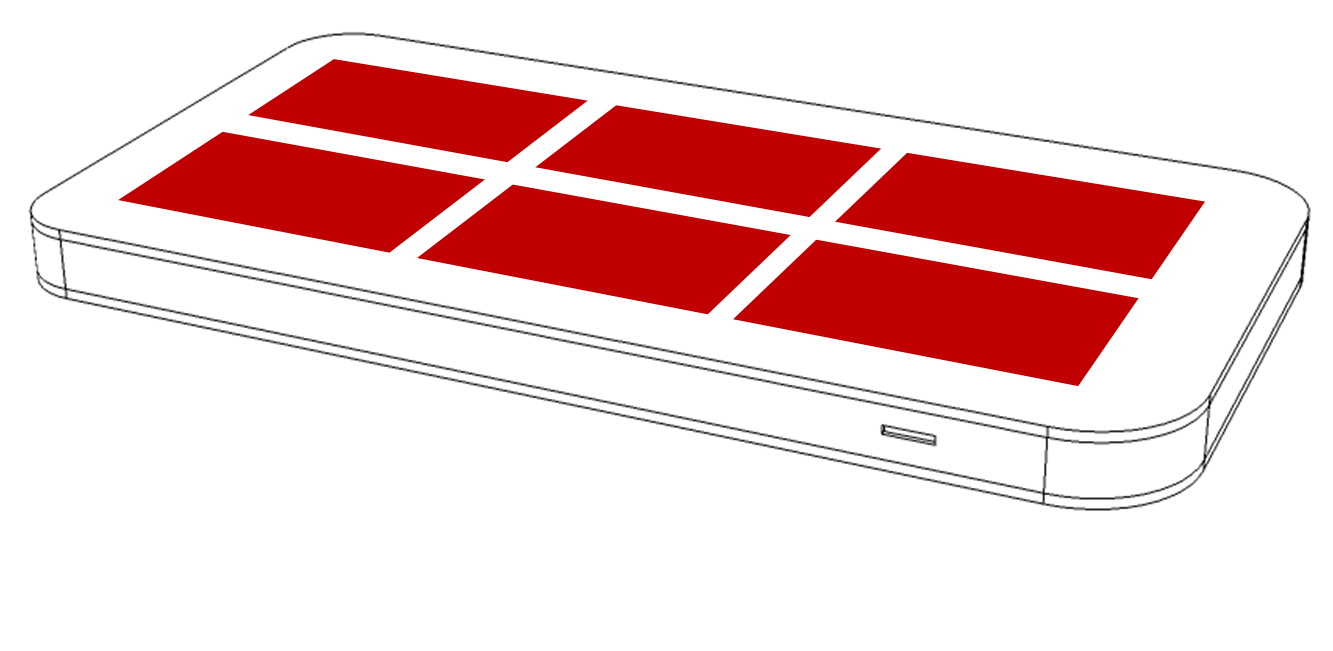
\includegraphics[width=0.6\textwidth]{images/magicbox}
\caption{MagicBox sketch - six electrodes uniformly distributed below surface}
\label{fig:magicbox_sketch}
\end{figure}
%Figure 28 MagicBox sketch - six electrodes uniformly distributed below surface
The so-called MagicBox was our first attempt to create an interaction device based on capacitive proximity sensing. It is using an array of six individual wireless capacitive sensors that communicate to a central station \cite{Braun2011MultiInputDevice}. The electrodes are using a large surface area and are made of aluminum foil. A sketch is shown in Figure \ref{fig:magicbox_sketch}. The system is able to track the position of a single hand in three dimensions up to a distance of approximately $20cm$, and uses different methods to infer gestures from the hand movement. 
It is designed to be a generic interaction device that can potentially be hidden below non-conductive surfaces. As it can be used without touching it is also applicable in sterile environments. A suite of demonstration applications has been created that showcase typical scenarios for the MagicBox. This includes multimedia applications, like image viewer and media player but also a 3D object viewer intended as demonstrator for potential medical applications, allowing a surgeon to check MRT or CT images in a sterile environment without touching any surface.
\subsection{Data processing}
 \begin{figure}[h]
\centering
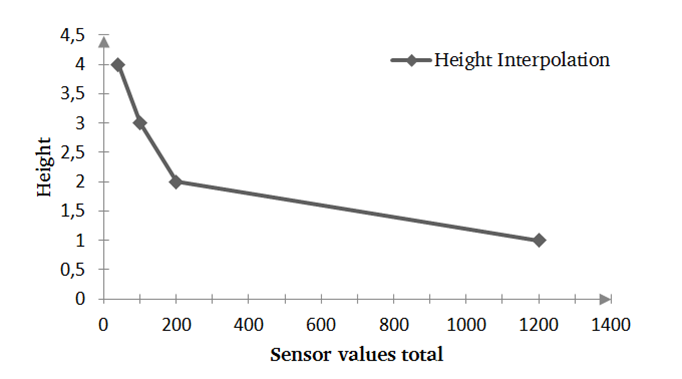
\includegraphics[width=0.6\textwidth]{images/magicbox_data_zaxis}
\caption{Piecewise linear hand distance estimation \cite{Braun2011MultiInputDevice}}
\label{fig:magicbox_data_zaxis}
\end{figure}
%Figure 29 Piecewise linear hand distance estimation [78]
The first data processing step of the MagicBox is the planar localization of the hand, following the weighted average algorithm previously presented. In order to calculate the distance of the hand from the plane we are using a piecewise linear interpolation, that resembles the response curve of a single sensor \cite{Braun2011MultiInputDevice}.
\begin{figure}[h]
\centering
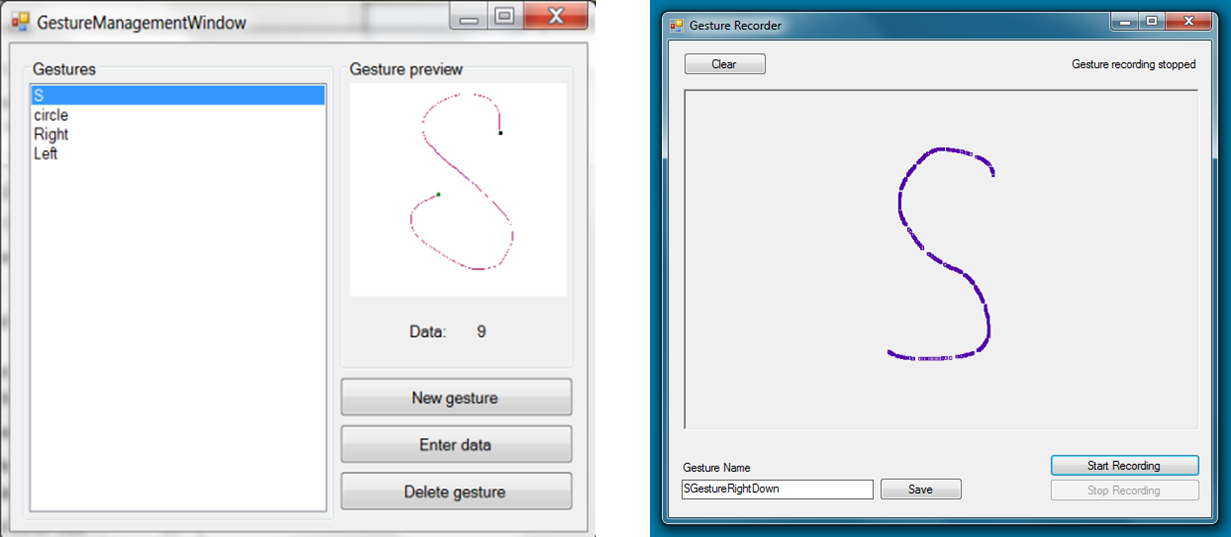
\includegraphics[width=0.7\textwidth]{images/magicbox_data_gest}
\caption{Gesture overview module (left) and gesture recorder (right)}
\label{fig:magicbox_data_gest}
\end{figure}
%Figure 30 Gesture overview module (left) and gesture recorder (right)
An addition of the MagicBox was a generic gesture recognition module based on methods similar to mouse gesture recognition \cite{braun2013capacitive}, albeit adapted for three dimensional locations. The developed debug software allows defining an arbitrary set of potential gestures and adding training data, as shown in Figure \ref{fig:magicbox_data_gest}. The module is looking for matches based on the most recent set of locations. 
\subsection{Evaluation}
\begin{figure}[h]
\centering
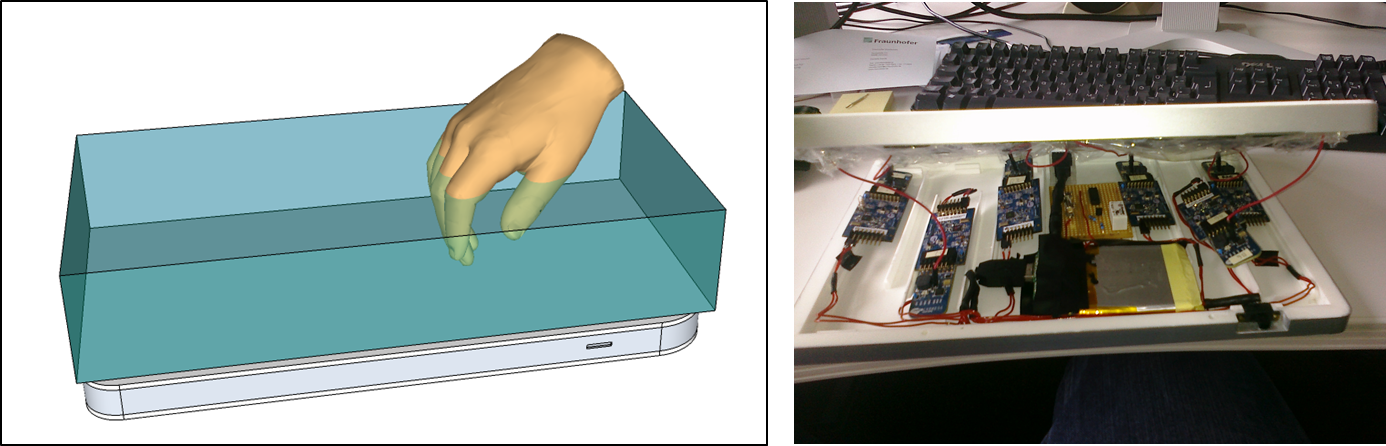
\includegraphics[width=0.8\textwidth]{images/magicbox_proto}
\caption{MagicBox conceptual rendering (left) and detail view of electronics (right) \cite{Braun2011MultiInputDevice}}
\label{fig:magicbox_proto}
\end{figure}
%Figure 31 MagicBox conceptual rendering (left) and detail view of electronics (right) [78]
The MagicBox prototype is based on the Cypress First Touch starter kit \cite{cypressfirst} and combines six capaci-tive sensors communicating wirelessly to a single base station, that are put together with a USB-rechargeable power supply into a casing. A concep-tual rendering showing the interaction area and a detail view of the prototype electronics are shown in Figure \ref{fig:magicbox_proto}.
\begin{figure}[h]
\centering
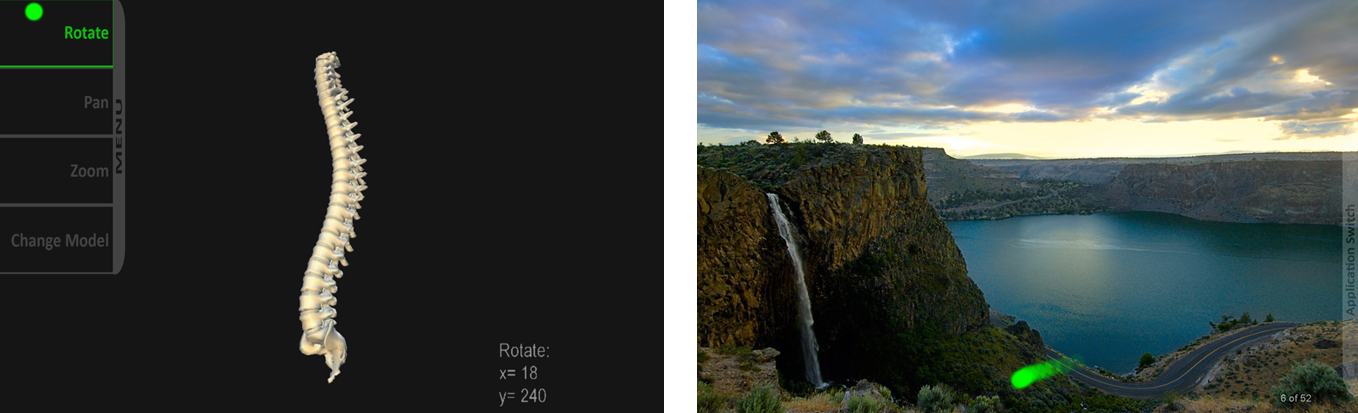
\includegraphics[width=0.8\textwidth]{images/magicbox_eval}
\caption{MagicBox demonstration application - 3D object viewer (left) and image viewer (right) \cite{Braun2011MultiInputDevice}}
\label{fig:magicbox_eval}
\end{figure}
%Figure 32 MagicBox demonstration application - 3D object viewer (left) and image viewer (right) [78]
The different iterations of the MagicBox have been evaluated in conjunction with various demon-stration applications. A usability study with 18 per-sons led to general approval of the system \cite{Braun2011MultiInputDevice}. Two of the applications used in this study are shown in Figure \ref{fig:magicbox_eval}. On the left is a 3D object viewer that has to be controlled by a combination of menu and direct manipulation of the screen content. On the right side there is an image viewer that was controlled by gesture to trigger the next/previous images or perform zooming operations. The most common positive remarks gathered in this study can be roughly put into three groups:
\begin{itemize}
\item{The device very intuitive to use}
\item{The idea of interacting this way is novel and interesting}
\item{It is easy to control applications with those gestures}
\end{itemize}
Likewise we identified three main groups for negative comments about the prototype:
\begin{itemize}
\item{The device is not very precise}
\item{The interaction speed is slow}
\item{It can be tiring for the arm}
\end{itemize}
Later iterations have been trying to improve some of the weaknesses presented above, e.g. by using a more sophisticated gesture recognition system and faster sensor refresh rates. Accordingly there were fewer complaints about interaction speed and precision \cite{braun2013capacitive}. However, the final complaint about the device being tiring for the arm, requires a different approach, that we are investigating in the final prototype to be presented in this system.
